\section{Reconfiguration Mechanism} \label{mechanism}

In this section we describe the reconfiguration protocol and the changes required to \LBFT protocol.
One of the design goal is to decouple these two protocols as much as possible to provide nice abstractions.
\begin{figure}[h]
			\centering
		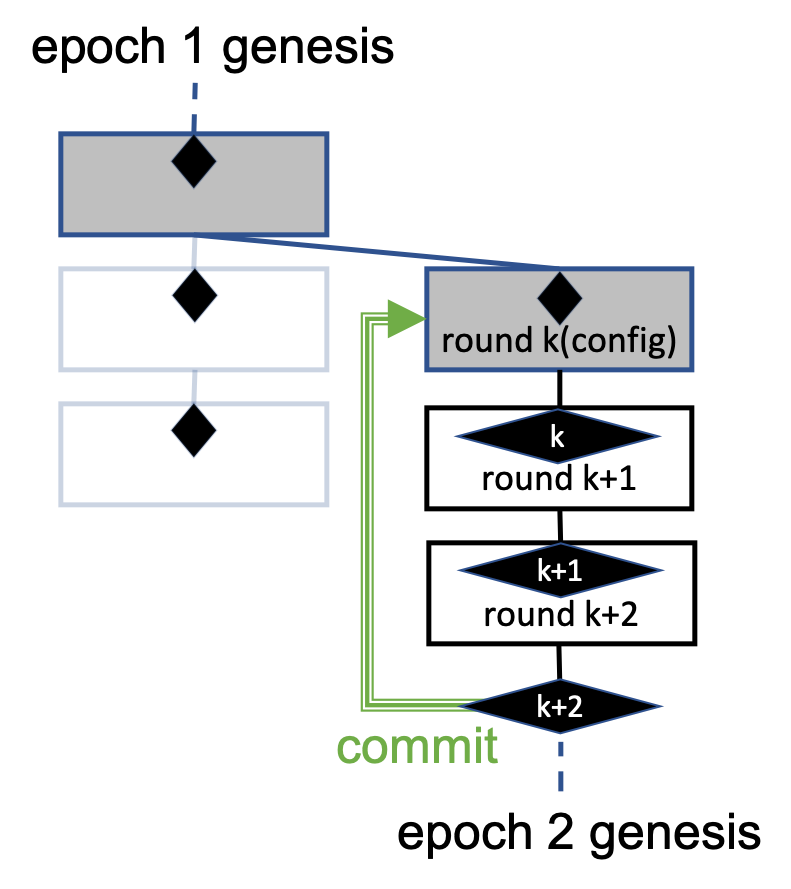
\includegraphics[scale=.45]{figures/reconfig1.png}
	\caption{Commit reconfig transaction}
\end{figure}

\subsection{Reconfiguration Protocol}

\emph{Epoch} is a monotonous increasing number used to refer to a \LBFT instance running with a specific configuration.
\LBFT instance is agnostic to epoch numbers, so we introduce \module{EpochManager} to process epoch related information.

\subsubsection{Message types}

First we add \emph{epoch} to every message types of \LBFT protocol including proposals, votes, timeout msg etc. Messages
with the same \emph{epoch} as local \LBFT protocol go to \LBFT for processing. Messages that have different \emph{epoch}
go to \rust{EpochManager.process\_different\_epoch\_messages}.

Additionally we introduce two messages types \rust{EpochChange} and \rust{EpochRetrieval}:

\begin{algorithm}[H]
\myalgorithm
{\SetAlgoNoLine
\tcp{The commit proof signed by \LBFT}
\Iblock{\rust{LedgerInfo}}{
	\rust{state\_id} ;\;
	\rust{signatures} ;\;
	... \;
	\rust{next\_configuration}: \rust{Option<Configuration>} ; \tcp{Added field to support reconfiguration}
}

\BlankLine
\tcp{Signals an \emph{epoch} change from $i$ to $j$}
\Iblock{\rust{EpochChange}}{
	\rust{start\_epoch} ; \tcp{The epoch of the first ledger info}
	\rust{end\_epoch} ; \tcp{The epoch after the last ledger info}
	\rust{proof}: \rust{Vec<LedgerInfo>} ;
}

\BlankLine
\tcp{Rquest an EpochChange from start\_epoch}
\Iblock{\rust{EpochRetrieval}}{
	\rust{start\_epoch} ;
}
}
\end{algorithm}

\subsubsection{EpochManager}
We have three different handlers for \module{EpochManager} to process those messages.

\paragraph{Handling different epoch, \rust{process\_different\_epoch\_msg}:}

When the different \LBFT epoch messages comes, we'll compare our local \emph{epoch} with the messages. If we're behind, we'll
issue a \rust{EpochRetrieval} to the peer who sent the message. If we're ahead, we'll provide
a \rust{EpochChange} to the peer.

\paragraph{Handling epoch retrieval, \rust{process\_epoch\_retrieval}:}
It's similar to how to process messages from lower \emph{epoch}, we'll provide the \rust{EpochChange} to help peer join our
\emph{epoch}.

\paragraph{Handling epoch change, \rust{start\_new\_epoch}:}

When we receive an \rust{EpochChange}, first we verify we're at \emph{epoch} $i$ and the \rust{EpochChange} is correct by iterating through the
ledger info and verify the signatures are corresponding to the configuration, then we ensure we're ready for the configuration of \emph{epoch}
$j$ e.g. sync to the ledger state at the beginning of the \emph{epoch} $j$. Finally we spawn a new \LBFT instance with
 the configuration of \emph{epoch} $j$.

\subsection{Changes to \LBFT}

Although \LBFT is agnostic to \emph{epoch}, it has to support additional rules for \textbf{reconfiguration protocol} in order to
maintain the safety property across \emph{epoch}.

\subsubsection{Commit Flow}
Just a kind reminder that \LBFT has three-phase commit rule - once we collects a QC for three contiguous rounds k, k+1, k+2, we commit the the block at round k
and all its prefix.

To support \rust{EpochChange} mentioned above, we need to add an optional field \rust{next\_configuration} to the \rust{ExecutedState}
which is only outputed when executing a reconfiguration transaction. Remember that \rust{LedgerInfo} carries the \rust{ExecutedState},
so that it contains such field and can serve as end-peoch proof.

Besides the normal commit flow in \LBFT which persists transactions in ledger state, we have an additional step to broadcast
\rust{EpochChange} to all the current validators if the \rust{LedgerInfo} carries next\_configuration. \module{EpochManager}
would then kick in and handle the \rust{EpochChange} message and spawn new \LBFT instance with next\_configuration and shutdown the current one.

\subsubsection{Descendants of Reconfig Block - Safety} \label{safety}

In this section, we explain the need to keep all the descendants of a reconfig-block empty of transactions until it's committed otherwise we might
have safety violation e.g. double spend.

The fundamental problem here is that \LBFT spreads the phase of the protocol(for every proposal) over 3 rounds i.e.\ pipelining.
When it comes to configuration, the proposal after reconfiguration transaction is under a different configuration with its
parent and the pipelining may not work anymore, we'll discuss more about this in section \ref{correctness}.

We use validators configuration as example, demonstrated in Figure~\ref{fig:safety}. Imagine we're at \emph{epoch} $1$ with
\rust{validators\{a1, a2, a3, a4\}}, and there's a reconfiguration transaction changes us to \rust{validators\{c1, c2, c3, c4\}}.
Reconfiguration transaction is included in B1, and a4 collects QC for B3 which has a ledger info(commit proof) of B1 but only unveils to \rust{c1,
c2, c3} but not \rust{a1, a2, a3}. \rust{c1, c2, c3} will start the new epoch and use B1 as its genesis while \rust{a1, a2, a3}
is going through another three rounds B4, B5, B6 and finally commit B4(which has B1 as its ancestor) and unveil it to \rust{c4}.
Now \rust{c4} thinks B4 is the genesis. If we have a double spend txn1, txn2 that txn1 committed with B4 and txn2 committed in B10 in
new \emph{epoch} $2$ with \rust{c1, c2, c3}, clients who query \rust{c1, c2, c3} would see the double spend compared with \rust{c4}.

\begin{figure}[ht]
			\centering
		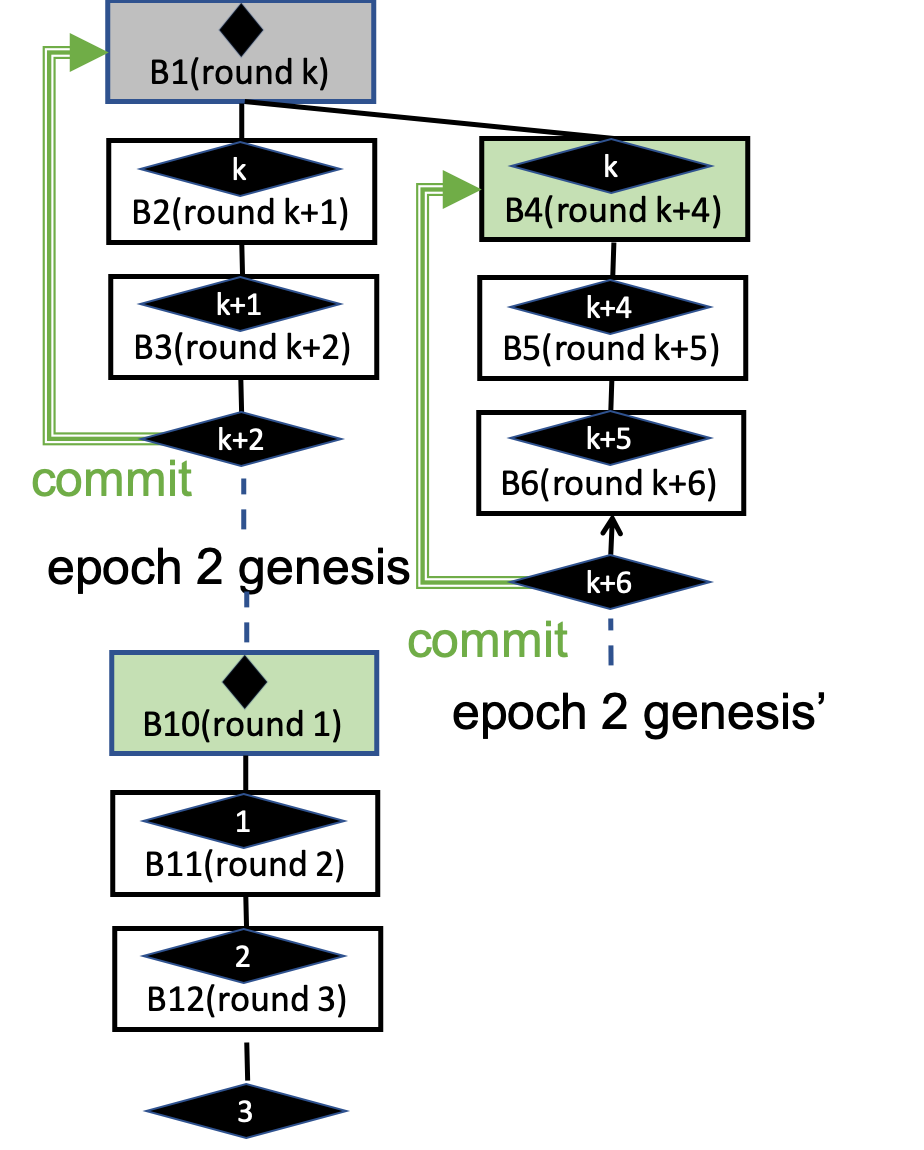
\includegraphics[scale=.45]{figures/reconfig-safety.png}
	\caption{Double spend in B4 and B10(green box)}
\label{fig:safety}
\end{figure}

Having any descendants of reconfiguration empty solves this problem, semantically it's equivalent to run 3 phases without
pipelining.

\subsubsection{Epoch Boundary - Liveness}
In this section, we explain how to specify the boundary of each \emph{epoch} and the risk of losing liveness if we don't do it correctly.
\paragraph{Start}
In \LBFT we assume everyone starts from a known genesis which we can consider as part of the configuration otherwise we'll lose liveness
even we preserve safety with empty blocks.
Intuitively we could use the block that includes reconfiguration transaction, but we may not commit that block directly but instead one
 of its descendants. And even worse, we may have multiple commit of its descendants since byzantine nodes could hide commits as Figure~\ref{fig:liveness}
 demonstrates.

\begin{figure}[ht]
	\centering
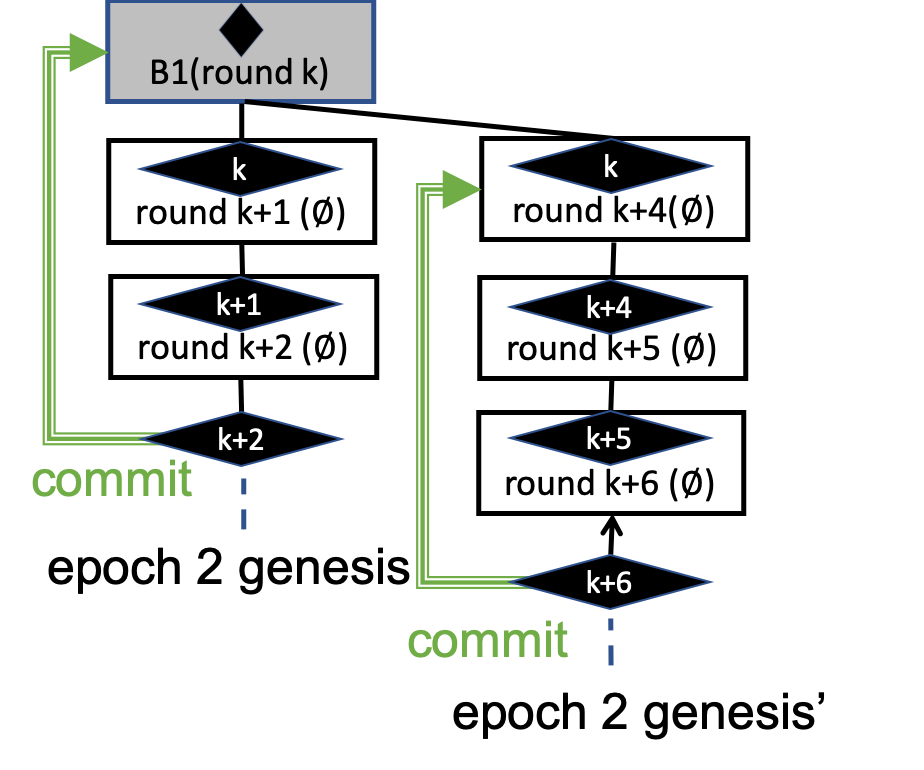
\includegraphics[scale=.45]{figures/reconfig-liveness.png}
\caption{If genesis is not equal to genesis', we lose liveness}
\label{fig:liveness}
\end{figure}

With the empty suffix blocks change, we ensure the same ledger state when we commit reconfiguration transaction regardless of which decendants,
and we leverage that to derive a genesis block so that every ledger info that ends previous \emph{epoch} would result in the same genesis deterministically.

\paragraph{End}
After a node sees \rust{LedgerInfo} that has \rust{next\_reconfiguration}, it'll stop participating the current \LBFT instance,
and spawning next \LBFT instance. If it's not part of the next reconfiguration, counterintuitively it can not shutdown itself
immediately otherwise we'll lose liveness. As an example, if we have \rust{validators\{a1, a2, a3, a4\}} at \emph{epoch} $i$, and
malicious \rust{a4} collects a \rust{LedgerInfo} and sends to \rust{a1} that's not part of \emph{epoch} $i+1$ and
\rust{a1} decides to shutdown itself. Byzantine node \rust{a4} also stops participating then \rust{a2, a3} would suffer a liveness problem and are never
able to make progress. To address such problem, \rust{a1} needs to keep the \rust{EpochManager} running until it sees a QuorumCert from new
\emph{epoch} so that it knows at least f+1 honest nodes in the new \emph{epoch} bootstrap.
